\documentclass{exam}
\usepackage{tikz}
\usepackage{subfig}
\usepackage{amsmath}
\usepackage[margin=1.0in]{geometry}
\pagestyle{empty}
\title{\textbf{Mock Test OMR Sheet}}
% \author{Author Name}
\date{\today}
\begin{document}
\maketitle
{\centering
Instructions for the exam should be here.}
 
\vspace{5mm}
 
\noindent\makebox[\textwidth]{Name:\enspace\hrulefill}
 
\vspace{5mm}

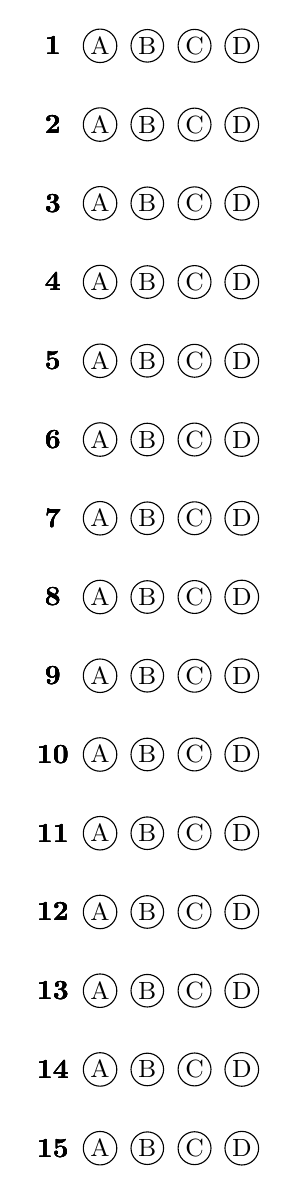
\begin{tikzpicture}[font=\small]
    \foreach \line in {1,2,...,15} {
        \begin{scope}[yshift=-\line cm]
            \foreach \letter/\position in {A/1, B/2, C/3, D/4} { 
                \node at (0,0) {\normalsize\textbf{\line}};
                \node[draw,circle,inner sep=1pt] at ({\position * 0.6},0) {\letter};
            }
        \end{scope}
    }
\end{tikzpicture}
\hfill
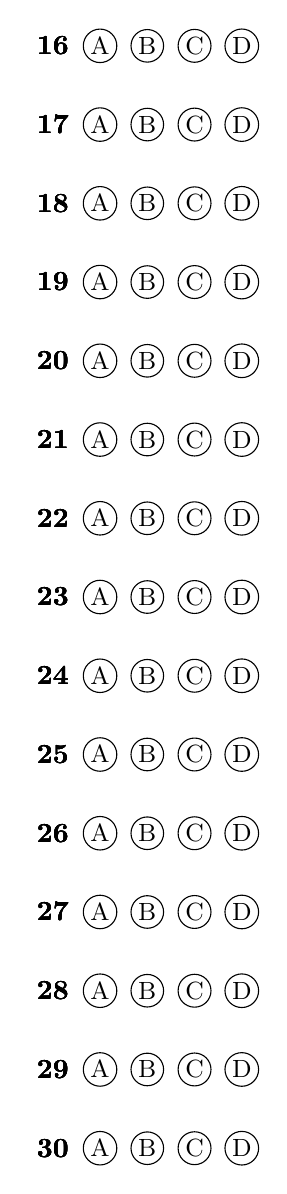
\begin{tikzpicture}[font=\small]
    \foreach \line in {16,17,...,30} {
        \begin{scope}[yshift=-\line cm]
            \foreach \letter/\position in {A/1, B/2, C/3, D/4} { 
                \node at (0,0) {\normalsize\textbf{\line}};
                \node[draw,circle,inner sep=1pt] at ({\position * 0.6},0) {\letter};
            }
        \end{scope}
    }
\end{tikzpicture}
\hfill
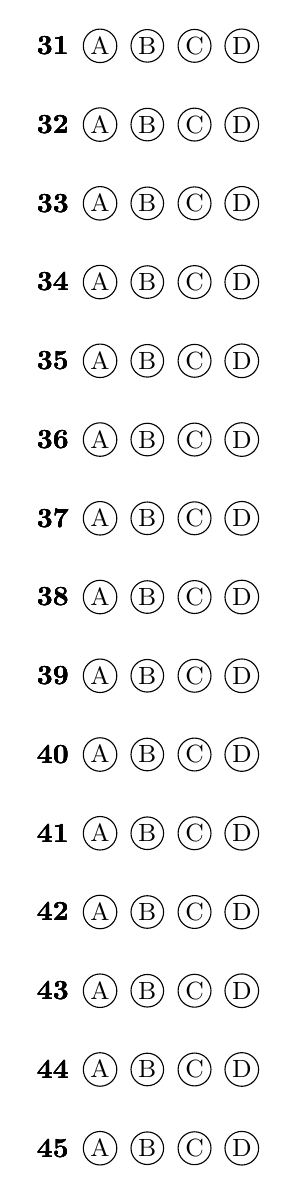
\begin{tikzpicture}[font=\small]
    \foreach \line in {31,32,...,45} {
        \begin{scope}[yshift=-\line cm]
            \foreach \letter/\position in {A/1, B/2, C/3, D/4} { 
                \node at (0,0) {\normalsize\textbf{\line}};
                \node[draw,circle,inner sep=1pt] at ({\position * 0.6},0) {\letter};
            }
        \end{scope}
    }
\end{tikzpicture}
\hfill
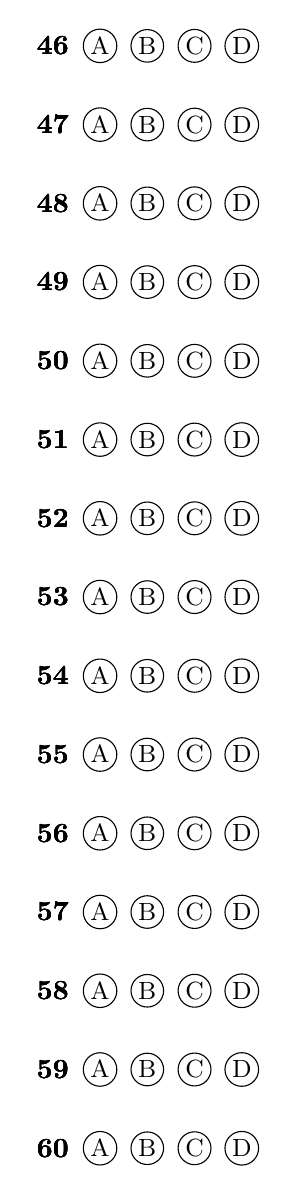
\begin{tikzpicture}[font=\small]
    \foreach \line in {46,47,...,60} {
        \begin{scope}[yshift=-\line cm]
            \foreach \letter/\position in {A/1, B/2, C/3, D/4} { 
                \node at (0,0) {\normalsize\textbf{\line}};
                \node[draw,circle,inner sep=1pt] at ({\position * 0.6},0) {\letter};
            }
        \end{scope}
    }
\end{tikzpicture}

\vfill

{\centering Correct Answers($\times$ 1) : \hrulefill Wrong Answers ($\times (-\frac{1}{4})$) : \hrulefill Total Marks : \hrulefill}
\end{document}